% !TeX program  = xelatex
% !TeX encoding = UTF-8
% !TeX root     = article1.tex
\documentclass{mirea-article}

% !TeX program  = xelatex
% !TeX encoding = UTF-8
% !TeX root     = article1.tex

\usepackage{hyperref}
\hypersetup{pdftitle={ВКР на тему "<Разработка системы для поиска и возврата утерянных вещей">}, pdfauthor={В. С. Верхотуров}}

\usepackage{comment}

\usepackage{graphicx}

\usepackage{listings}
\usepackage{xcolor}
\lstset{basicstyle=\footnotesize, breaklines=true, numbers=left, captionpos=t, showstringspaces=false, commentstyle=\color{teal}, stringstyle=\color{red}, keywordstyle=\color{violet}}  % Настройки, применяемые ко всем листингам

% Создание введения или заключения
\newcommand{\supersection}[1]{
	\section*{#1}
	\phantomsection
	\addcontentsline{toc}{section}{#1}
}

\usepackage{caption}
\captionsetup[lstlisting]{justification=raggedright, singlelinecheck=false}

\usepackage{pdfpages}

\usepackage{microtype}

\usepackage{multirow}

\usepackage{array}
\usepackage{setspace}
\newcolumntype{x}[1]{>{\setstretch{0.8}\small\centering\arraybackslash\hspace{0pt}}m{#1}}
\newcolumntype{y}[1]{>{\centering\arraybackslash\hspace{0pt}}m{#1}}
\usepackage{longtable}

\usepackage{float}

%\usepackage{color,xesearch}
%\SearchList{make-red}{\textcolor{red}{#1}}{эффективность,эффективности,эффективностью,эффективностей,эффективностям,эффективностями,эффективностях,эффективный,эффективная,эффективное,инновационный,иновационная,иновационные,инновация,иновационных,надежность,оптимизация,качество}

\usepackage{multicol}
\usepackage{ragged2e}

\newenvironment{Figure}
{\par\medskip\noindent\minipage{\linewidth}}
{\endminipage\par\medskip}

\begin{document}
	
	\textbf{УДК 004.658.2}
	
	\begin{FlushRight}
		\textbf{Валерий Сергеевич Верхотуров} 
		
		Студент специальности «Информационные системы и технологии» ИКБ РТУ МИРЭА valery.verkhoturov1505@gmail.com

		\textbf{Игорь Денисович Котилевец} 
		
		Научный руководитель, старший преподаватель кафедры ИКБ РТУ МИРЭА
	\end{FlushRight}
	
	\supersection{Сравнительный анализ существующих цифровых решений в сфере поиска потерянных вещей.} 
	
	Аннотация. \textit{Отслеживание пропавших предметов остается важной задачей, которая появляется в разнообразных ситуациях. Эта проблема может произойти из-за утери таких вещей, как ключи, удостоверения личности, смартфоны, бумажники или другие предметы значимости или необходимости. Поэтому актуален вопрос о разработке систем, способных помочь людям находить потерянное. Данная статья освещает обзор текущих методик и систем, предназначенных для поиска утраченных предметов.}
	
	Ключевые слова: \textit{бюро находок, веб-сайт, RFID, GPS.}
	
	\supersection{A comparative analysis of existing digital solutions in the field of lost items retrieval}
	
	Annotation. \textit{Tracking missing items remains an important task that arises in a variety of situations. This problem can occur due to the loss of items such as keys, ID cards, smartphones, wallets, or other items of significance or necessity. Therefore, the issue of developing systems that can help people find what they have lost is relevant. This article provides an overview of current techniques and systems designed to locate lost items.}
	
	Keywords: \textit{lost and found, websit, RFID, GPS.}
	
	\subsection*{Введение}
	\label{sec:introduction}
	
	Поиск утерянных вещей является актуальной проблемой, которая возникает при различных обстоятельствах. Эта проблема может возникнуть в результате потери ключей, документов, мобильных телефонов, кошельков или других ценных или важных вещей~\cite{bib:m24_losts_article,bib:usinsk_losts_article}. В связи с этим существует необходимость разработки системы, которая поможет людям вернуть утерянные вещи.
	
	\subsection*{Статистика потерянных и найденных вещей}
	
	Для подтверждения актуальности и важности сравниваемых систем, необходимо провести исследование рынка и определить основные проблемы и потребности пользователей. Одним из способов сбора информации является проведение опроса среди пользователей.
	
	Одним из основных факторов, определяющих актуальность разрабатываемой системы является статистика потерянных и найденных вещей. Необходимо определить количество потерянных вещей в месяц, год и за весь период работы системы. Это поможет оценить нагрузку на систему и определить ее производительность.
	
	Статистика, взятая с сайта столнаходок.рф~\cite{bib:stol_nahodok}, утверждает, что только 20~\% пользователей их сайта смогли установить и вернуть вещи. Также на рисунках \ref{fig:chart2023} и \ref{fig:chart2022} представлена гистограмма количества созданных объявлений за 2022 и 2023 года.
	
	\begin{Figure}
		\centering
		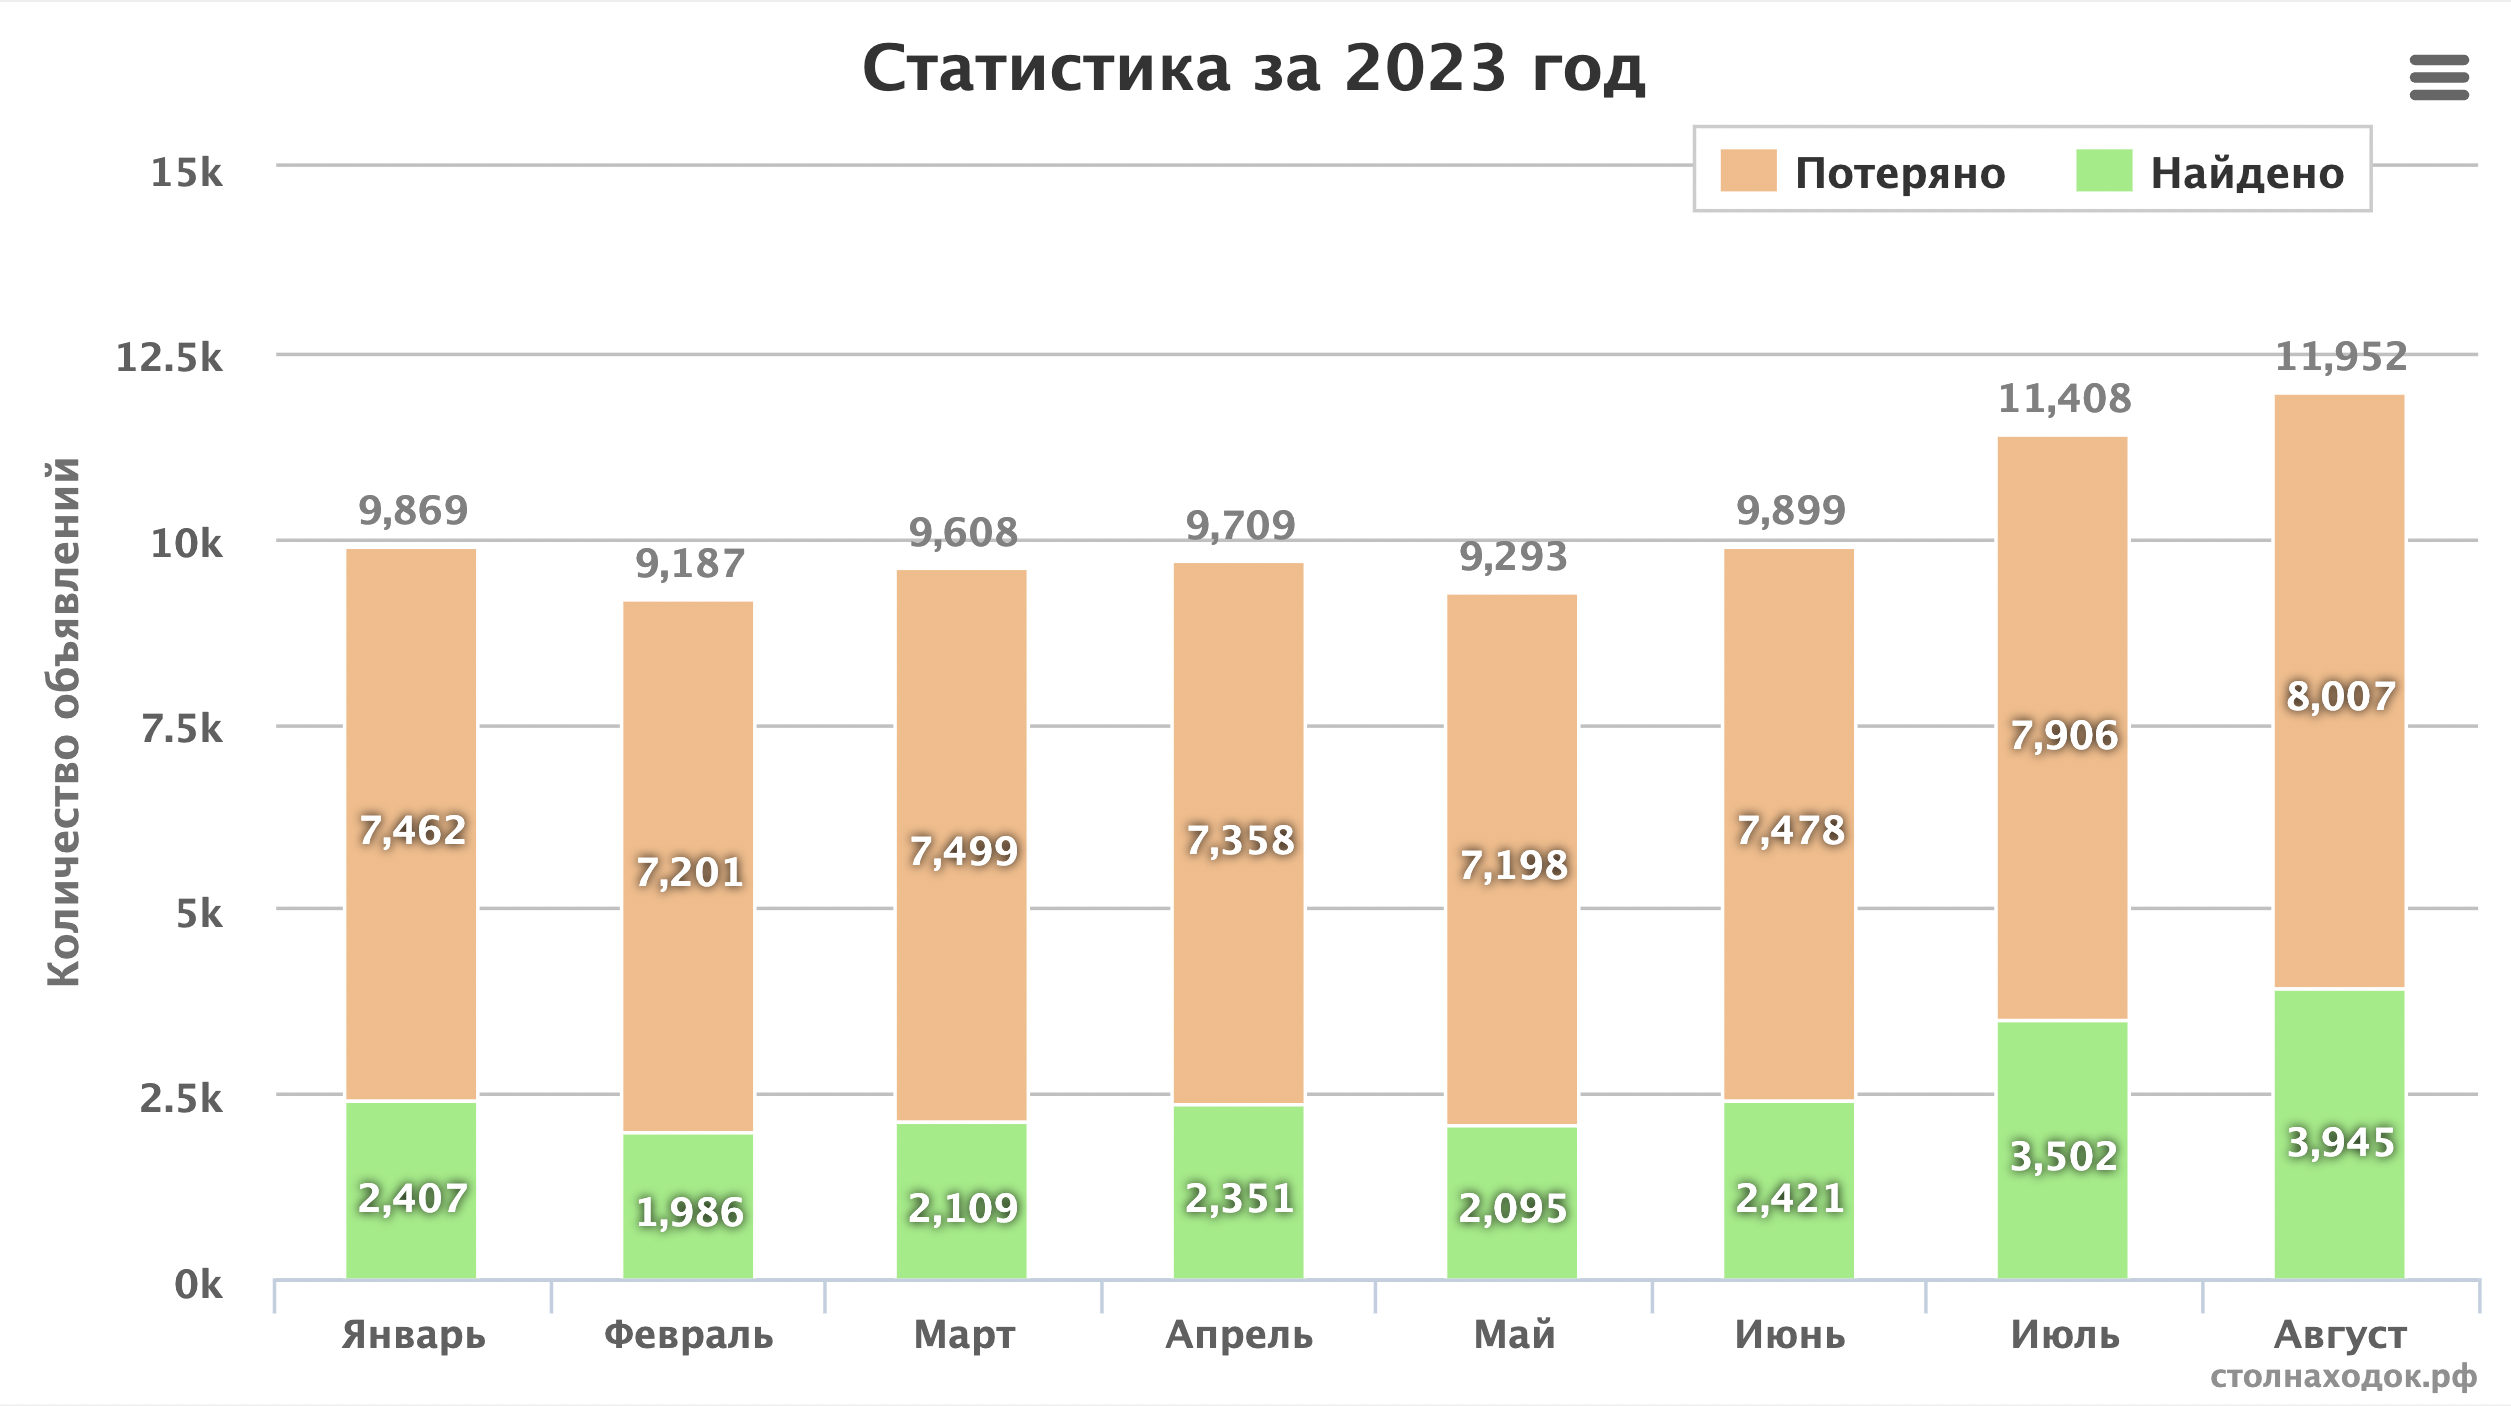
\includegraphics[width=\textwidth]{../images/chart2023}
		\captionof{figure}{Востребованность системы столнаходок.рф в 2023 году}
		\label{fig:chart2023}
	\end{Figure}
	
	\begin{Figure}
		\centering
		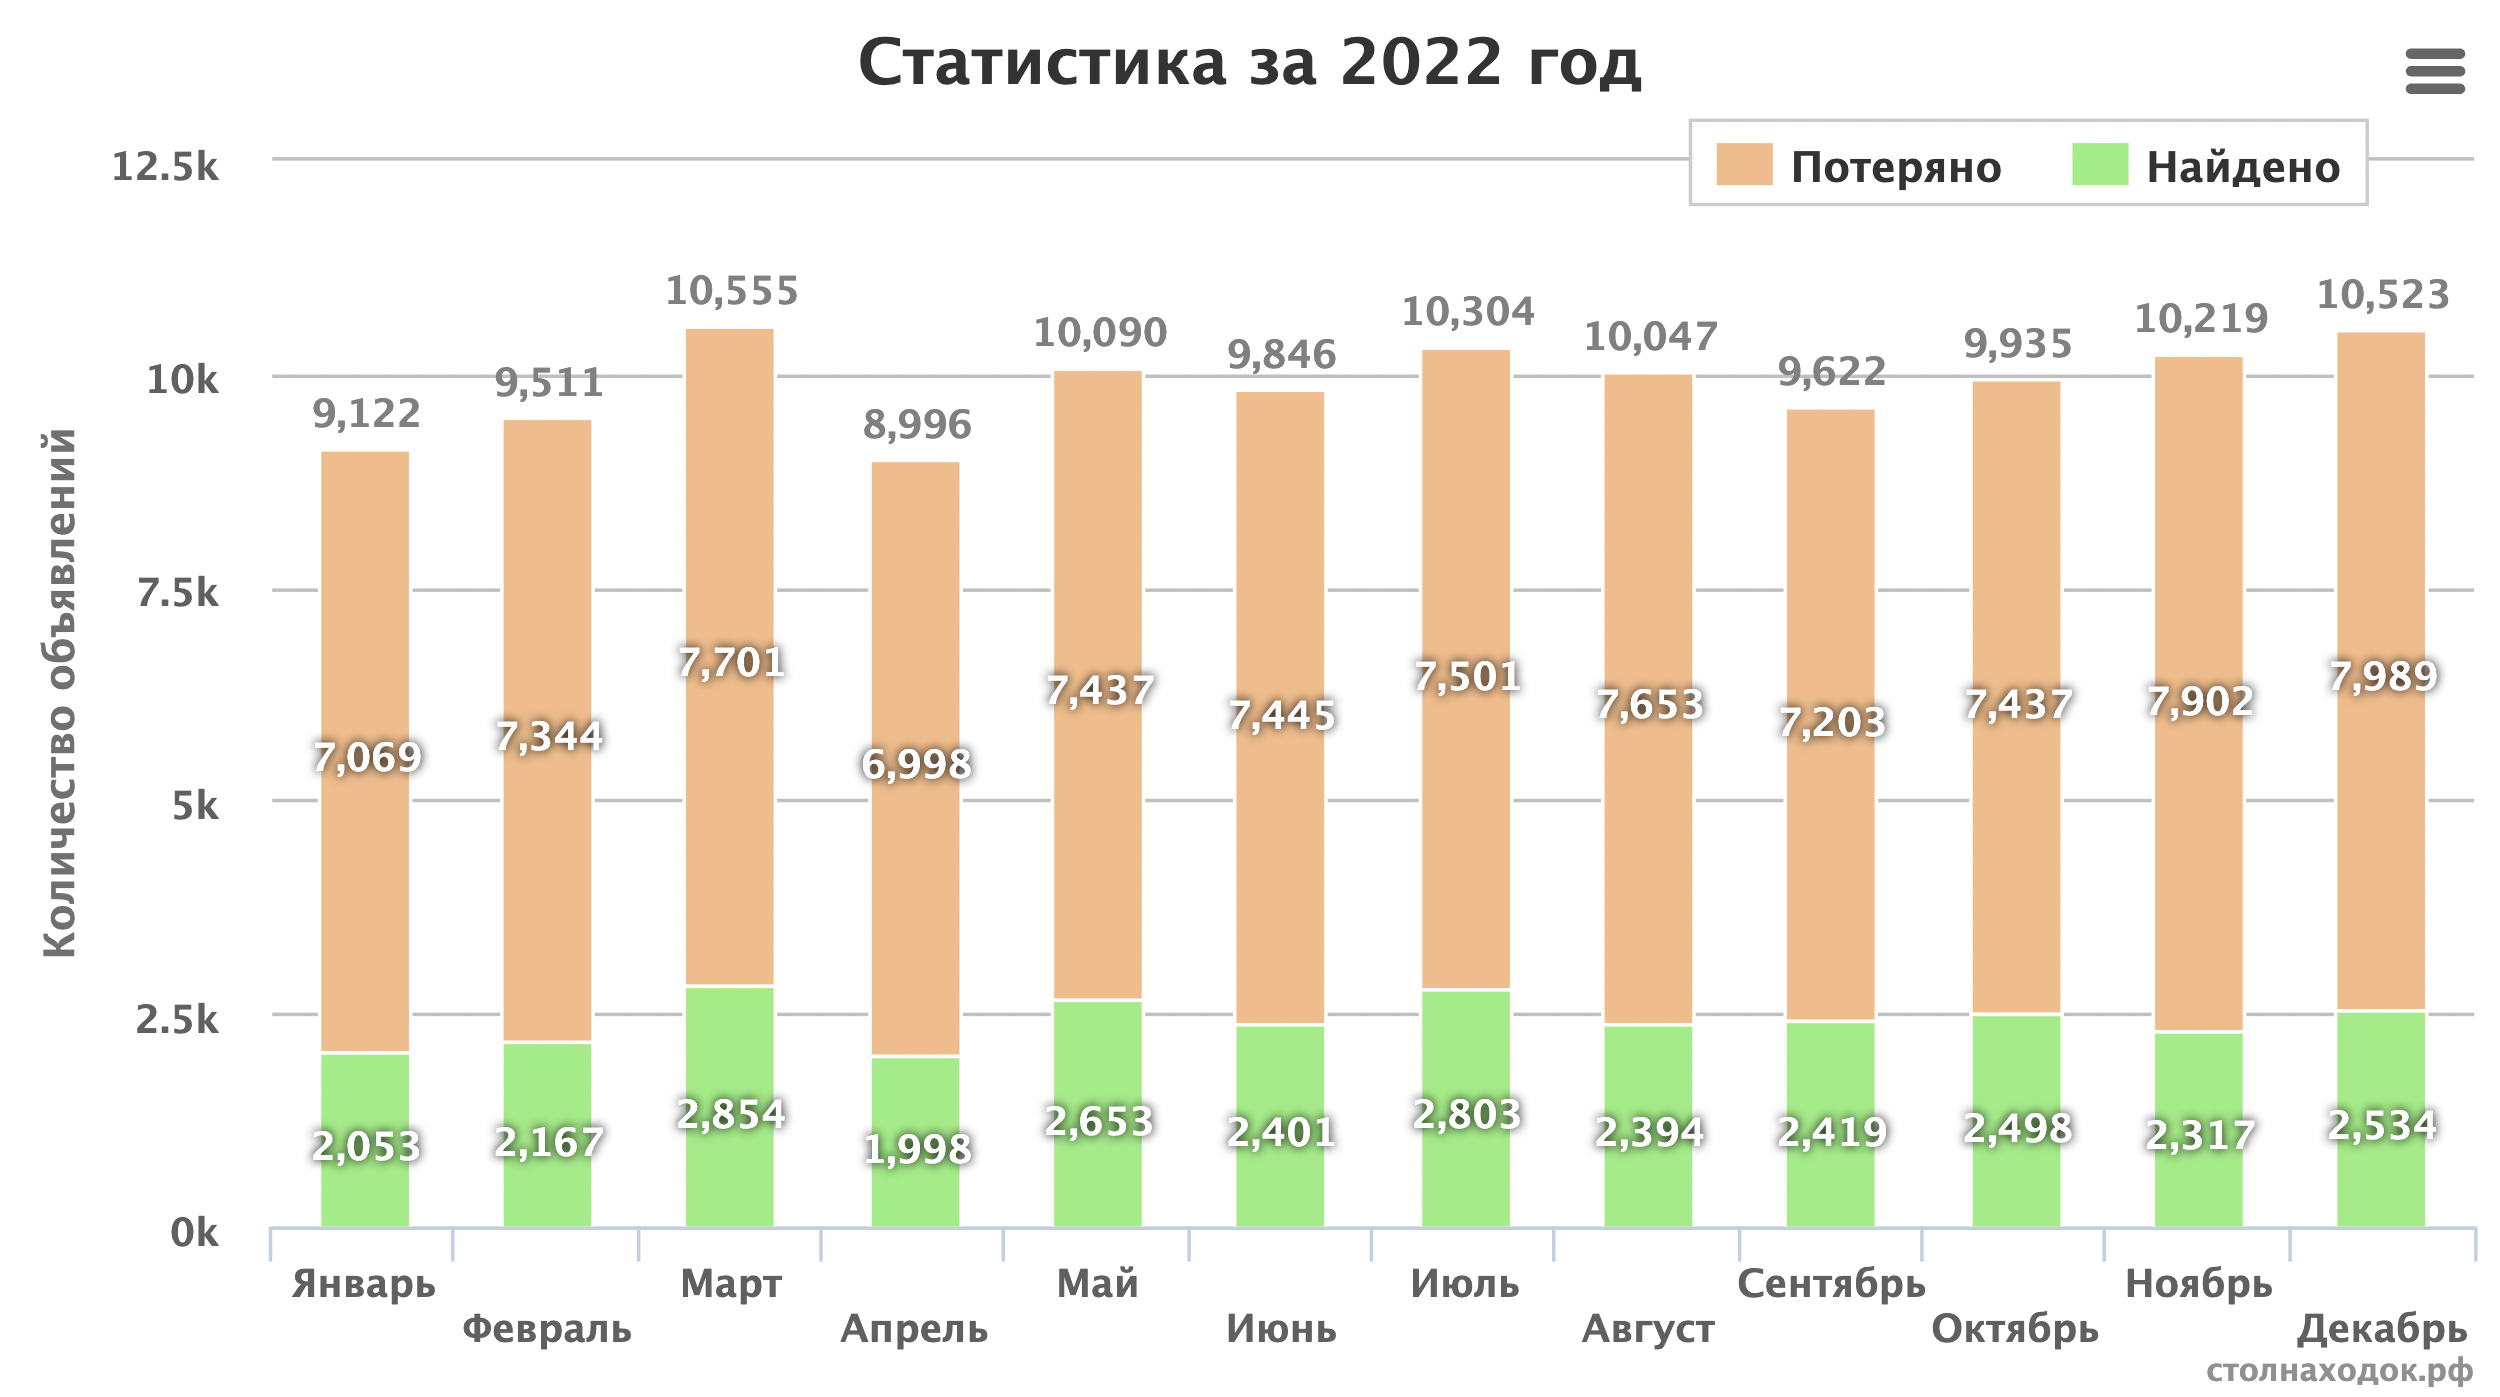
\includegraphics[width=\textwidth]{../images/chart2022}
		\captionof{figure}{Востребованность системы столнаходок.рф в 2022 году}
		\label{fig:chart2022}
	\end{Figure}
	
	\subsection*{Типы существующих решений для поиска и возврата утерянных вещей}
	
	Существует несколько типов существующих решений для поиска и возврата утерянных вещей. Ниже приведены некоторые из них:
	\begin{enumerate}
		\item Веб-сайты и мобильные приложения: <<Бюро находок>>~\cite{bib:stol_nahodok,bib:pona}. Эти сервисы предоставляют платформу, где люди могут регистрировать утерянные вещи и искать их владельцев. Пользователям предлагается создать объявления о найденных или потерянных вещах и связаться друг с другом, чтобы вернуть вещи. Некоторые сервисы предлагают добавить фотографии или описание вещей, чтобы облегчить поиск. 
		
		\item Технология RFID (Radio Frequency Identification) позволяет прикреплять RFID-метки к ценным объектам и определить владельца с помощью специальных считывателей~\cite{bib:investopedia_rfid,bib:airtag}. Это возможно благодаря использованию радиоволн, которые позволяют быстро определять местоположение потерянных вещей с помощью дополнительного программного обеспечения. Одним из наиболее распространенных применений технологии RFID является микрочипирование домашних животных или чипов для домашних животных. Эти микрочипы имплантируются ветеринарами и содержат информацию, касающуюся домашних животных, включая их имя, медицинские записи и контактную информацию их владельцев. Если домашнее животное пропадает и его отправляют в спасательную службу или в приют, работник приюта сканирует животное на наличие микрочипа. Если у домашнего животного есть микрочип, работнику приюта достаточно одного телефонного звонка или поиска в Интернете, чтобы связаться с владельцами домашнего животного. Считается, что чипы для домашних животных более надежны, чем ошейники, которые можно упасть или снять.
		
		\item GPS-трекеры --- это устройства с встроенным GPS-модулем. Они могут быть прикреплены практически к любому объекту, после чего его местоположение определяется через смартфон или компьютер по сети Интернет. При использовании приложения на смартфоне пользователь может получать уведомления о передвижении объекта и быстро определять его текущее местоположение.
		
		\item Автоматизированные системы поиска утерянных предметов: Некоторые организации, например, аэропорты и железнодорожные станции, используют системы обнаружения утерянных предметов. В этих системах используются технологии, такие как видеонаблюдение, детекторы движения и распознавание образов для отслеживания и возвращения потерянных предметов их владельцам.
	\end{enumerate}
	
	Каждый из этих типов решений имеет свои преимущества и недостатки. Некоторые из них могут быть более подходящими для конкретных ситуаций, например, GPS-трекеры могут быть полезными при поиске утерянных вещей на открытой местности, в то время как RFID-метки могут быть более подходящими для использования внутри помещений. Веб-сайты и приложения <<Бюро находок>> предоставляют более универсальное решение, которое может быть использовано в различных ситуациях.
	
	\subsection*{Анализ существующих систем для поиска и возврата утерянных вещей}
	
	В настоящем разделе будет проведен обзор существующих сервисов и приложений, которые предлагают функциональность поиска и возврата утерянных вещей. Данный обзор позволит выявить основные преимущества и недостатки этих сервисов, а также определить потенциальные возможности для улучшения их функциональности.
	
	<<столнаходок.рф>>~\cite{bib:stol_nahodok} --- это один из наиболее популярных веб-сервисов, предоставляющих возможность объявлять о потерянных и найденных предметах. Сервис имеет простой и интуитивно понятный интерфейс, позволяющий пользователям быстро разместить информацию о потерянных вещах и связаться с владельцами найденных предметов, примеры пользовательского интерфейса представлены на рис.~\ref{fig:stolNahodok1}, \ref{fig:stolNahodok2}. Однако, отсутствие системы уведомлений и неудобное сопоставление объявлений ограничивают его функциональность.
	
	\begin{Figure}
		\centering
		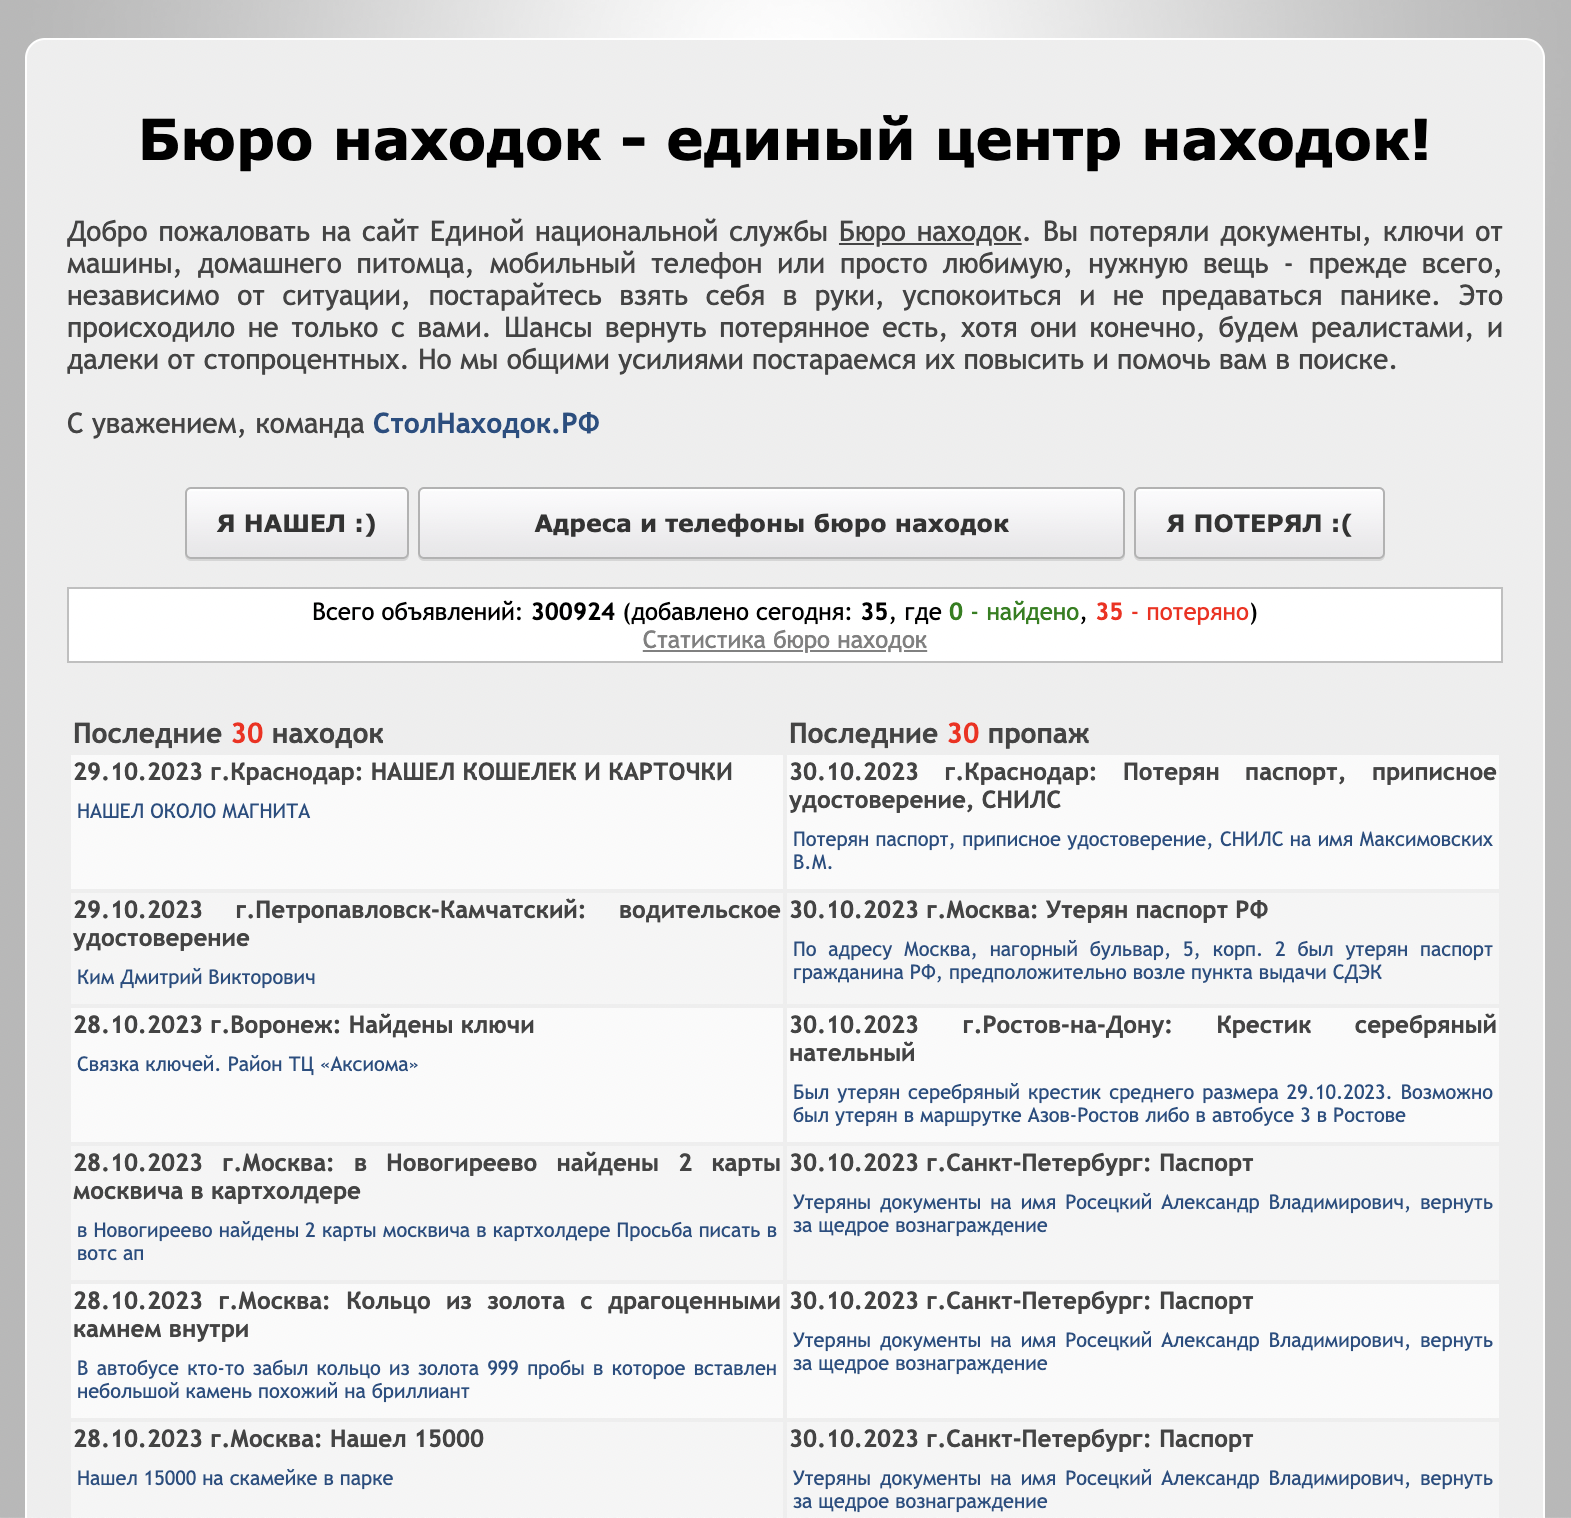
\includegraphics[width=0.5\textwidth]{../images/stolNahodok1}
		\captionof{figure}{Скриншот системы <<столнаходок.рф>>}
		\label{fig:stolNahodok1}
	\end{Figure}
	
	<<Find My Stuff>>~\cite{bib:stol_nahodok} --- это мобильное приложение, разработанное для операционных систем iOS и Android. Оно предлагает функцию отслеживания утерянных предметов через GPS-модуль смартфона, представлено на рис.~\ref{fig:findMyStuff1}. Пользователи могут отмечать свои вещи на карте и получать уведомления, когда они находятся рядом с утерянным предметом. Однако, ограничение использования только наличием смартфона с GPS-модулем и низкая точность определения местоположения представляют существенные ограничения данного приложения.
	
	\begin{Figure}
		\centering
		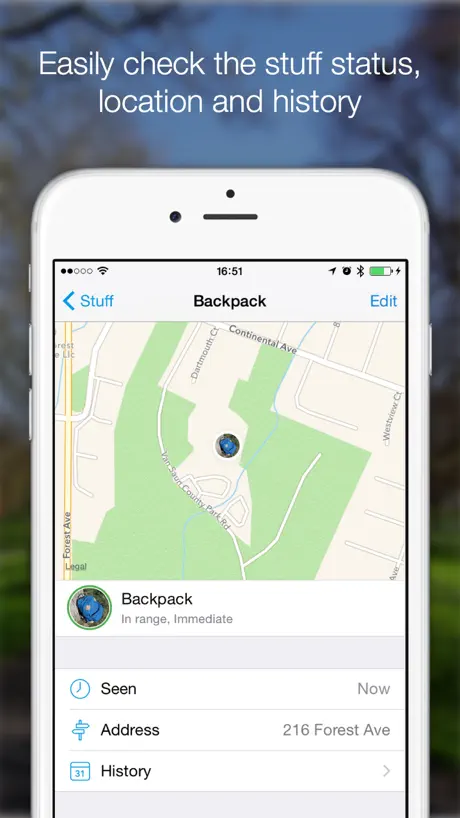
\includegraphics[height=.5\textwidth]{../images/findMyStuff1.png}
		\captionof{figure}{Скриншот системы <<Find My Stuff>>}
		\label{fig:findMyStuff1}
	\end{Figure}
	
	<<Lost Property Office>>~\cite{bib:parliament_lost_and_found} --- это веб-сервис, предоставляемый государственными организациями и органами правопорядка, см. рис.~\ref{fig:lostPropertyOffice}. Сервис позволяет пользователям сообщать о потерянных и найденных предметах, а также предоставляет информацию о процедуре возврата утерянных вещей. Однако, ограниченный доступ к сервису и неудобный процесс регистрации и подачи заявки являются значительными недостатками данного сервиса.
	
	\begin{Figure}
		\centering
		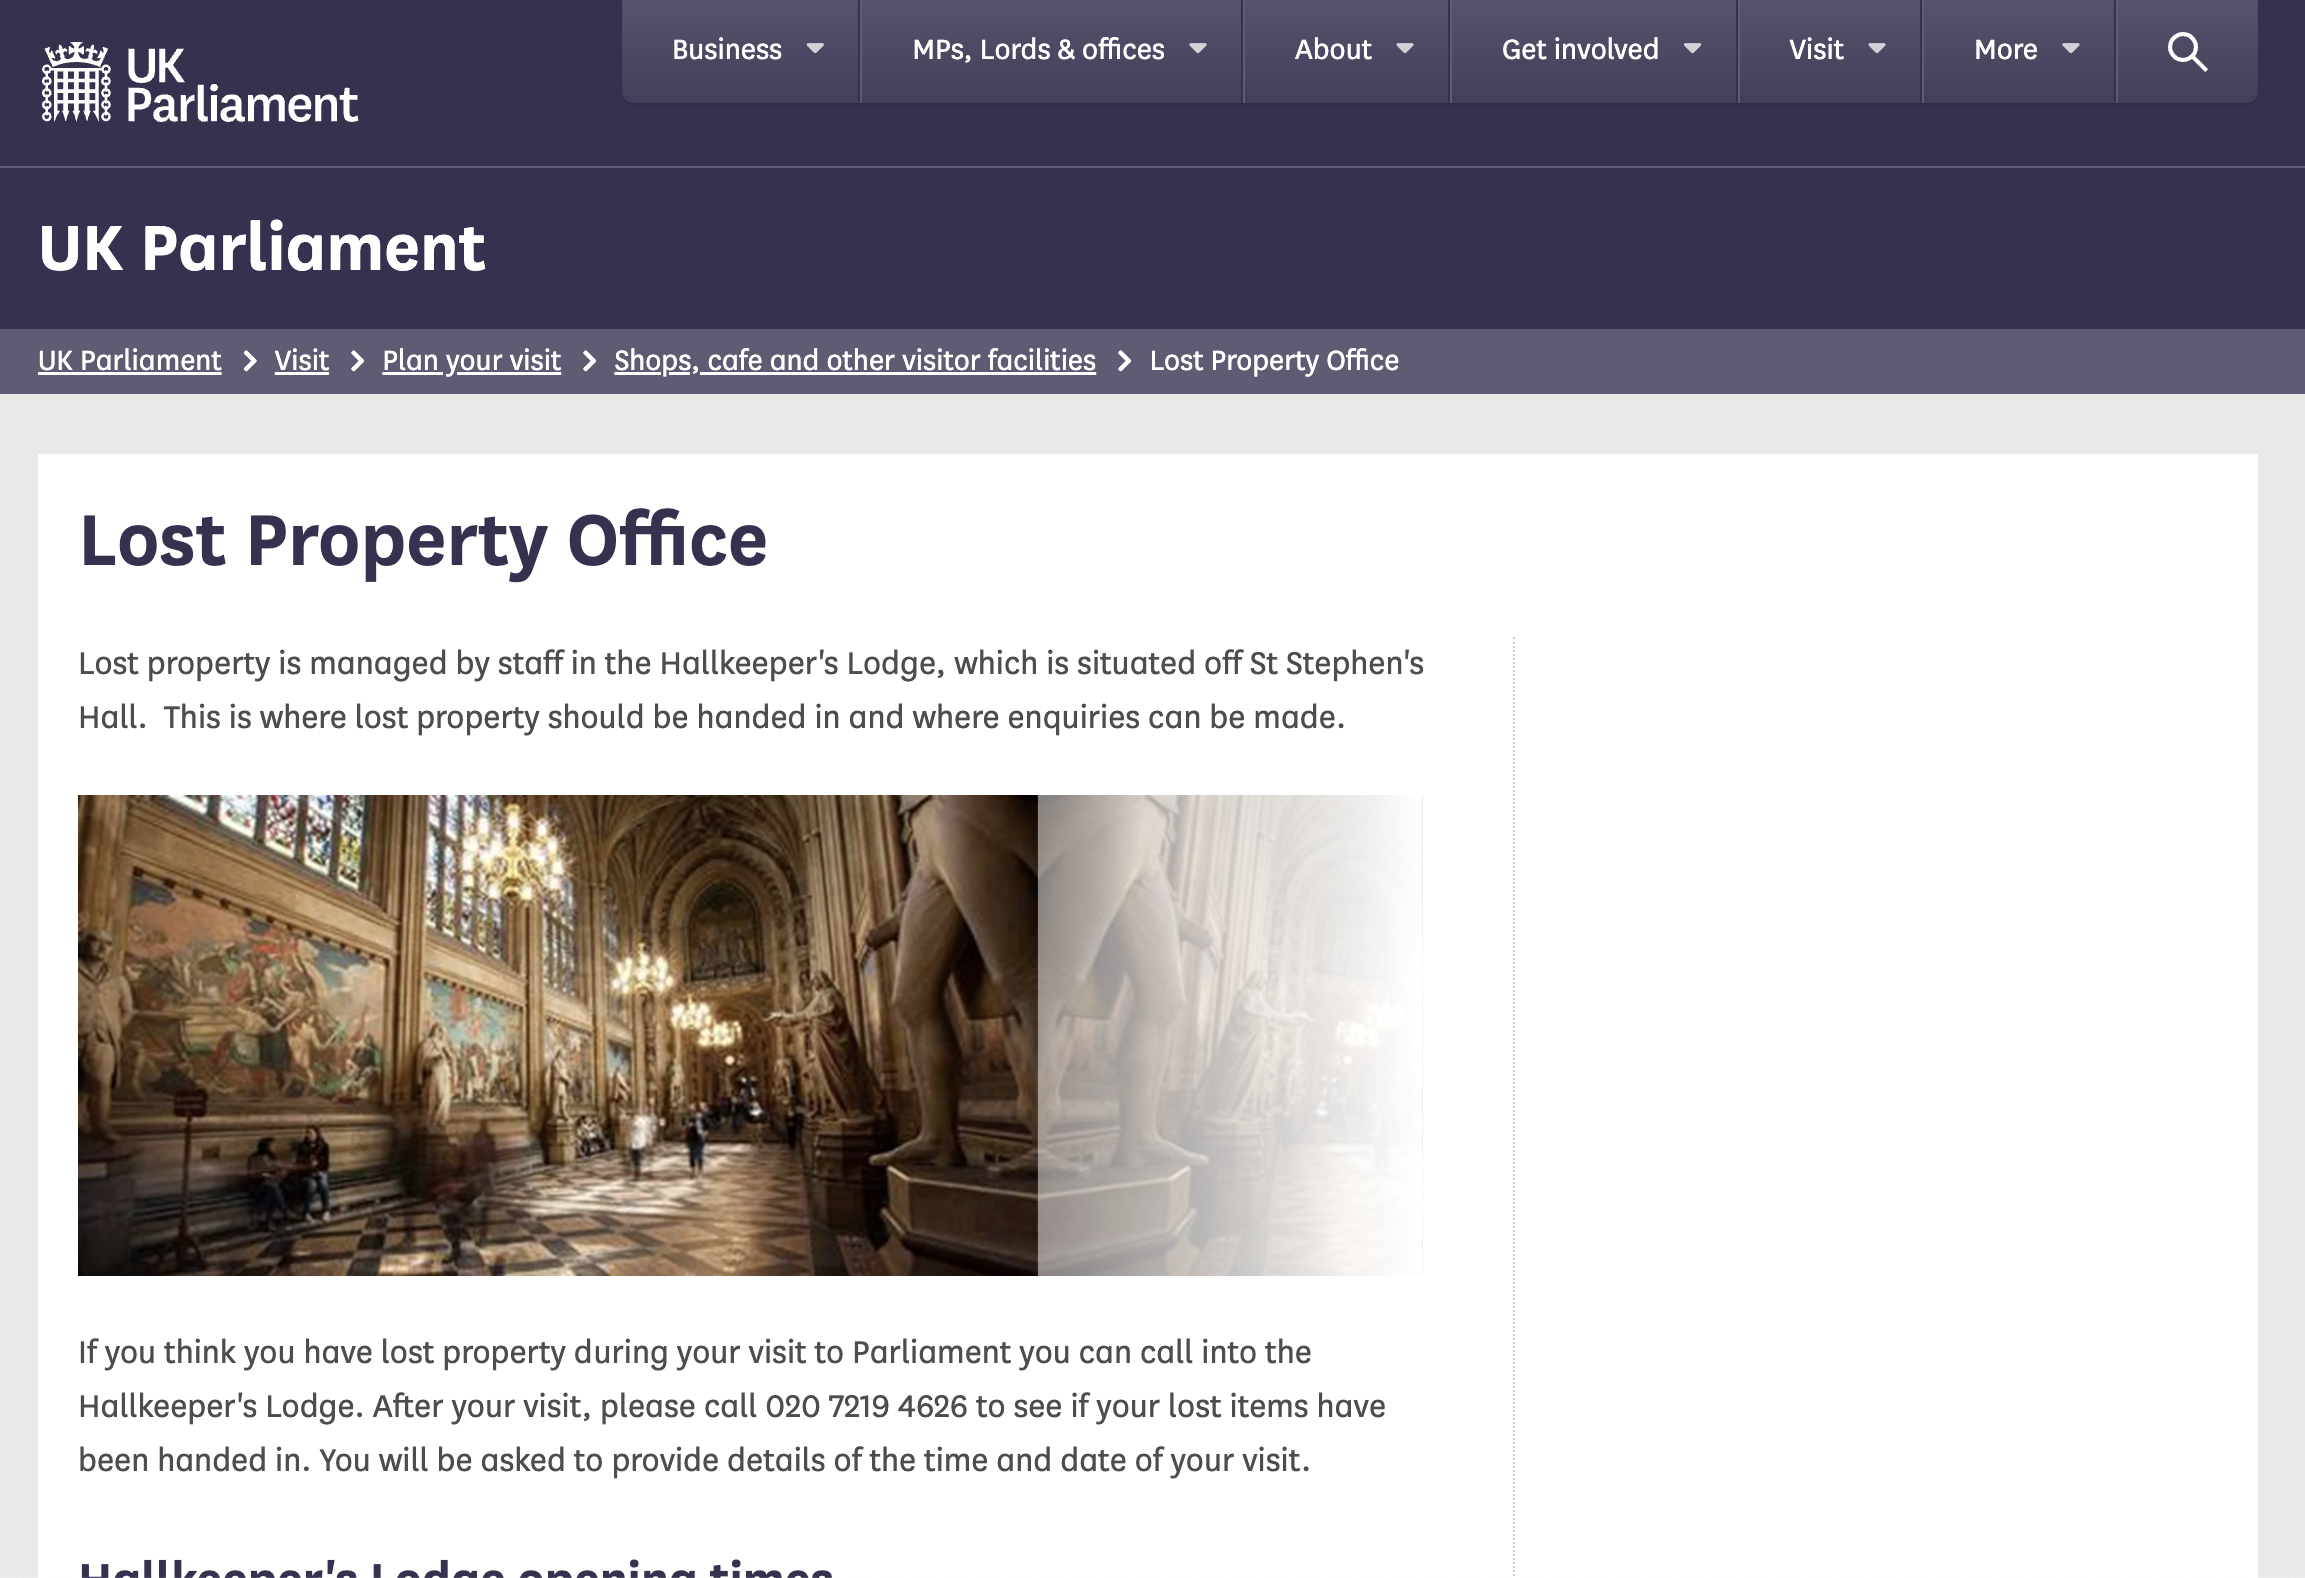
\includegraphics[width=.5\textwidth]{../images/lostPropertyOffice}
		\captionof{figure}{Скриншот системы <<Lost Property Office>>}
		\label{fig:lostPropertyOffice}
	\end{Figure}

	
	\begin{table}[htb]
		\caption{Сравнительный анализ систем по 10-бальной системе}
		\centering
		
		\tolerance=0
		\emergencystretch=10pt
		\hyphenpenalty=0
		\exhyphenpenalty=0
		\begin{tabular}{ | m{10em} | m{10em}| m{10em} | } 	
			\hline
			столнаходок .рф & Find My Stuff & Lost Propery Office \\ 
			\hline
			Устаревший UI (5 балла) & Удобный UI/UX (7 баллов) & Неудобный UI/UX (3 балла) \\ 
			\hline
			Нет уведомлений (0 баллов) & Есть push оповещения (10 аллов) & Нет уведомлений (0 баллов) \\ 
			\hline
			Широкий доступ (10 баллов) & Только через GPS (3 балла) & Ограничен\-ный доступ (5 баллов) \\ 
			\hline
			Итого --- 15 баллов & 20 баллов & 8 баллов \\ 
			\hline
		\end{tabular}
	\end{table}
	
	\subsection*{Вывод}
	
	В статье проведен детальный анализ существующих веб-ресурсов и приложений, предназначенных для поиска и возвращения утерянных вещей. Были изучены и проанализированы их функциональность, характеристики, преимущества и ограничения.
	
	Одним из наиболее популярных и востребованных решений в данной сфере являются веб-сервисы и приложения "Бюро находок". Они предоставляют пользователям платформу для регистрации утерянных вещей и связи с их владельцами, что упрощает процесс поиска и возвращения потерянных предметов.
	
	\begin{thebibliography}{99\kern\bibindent}
		\bibitem{bib:m24_losts_article} МОСКВА 24 Что теряют москвичи // www.m24.ru: Новости Москвы, репортажи и интервью об основных событиях города URL: \url{https://www.m24.ru/news/gorod/28112019/98853} (дата обращения: 01.09.2023).
		
		\bibitem{bib:usinsk_losts_article} Усинск Онлайн Какие вещи чаще всего теряют россияне // usinsk.online (дата обращения: 01.09.2023).
		
		\bibitem{bib:about1} Bataineh, Emad, Bilal Bataineh, and Shama Al Kindi. "Design, development and usability evaluation of an online web-based lost and found system." International Journal of Digital Information and Wireless Communications 5.2 (2015): 75-82. % https://citeseerx.ist.psu.edu/document?repid=rep1&type=pdf&doi=c757d2b9e8b8ba4235342217fab983e2f89f6bd0
		
		\bibitem{bib:about2} Tan, Siok Yee, and Cia Rui Chong. "AN EFFECTIVE LOST AND FOUND SYSTEM IN UNIVERSITY CAMPUS." Management 8.32: 99-112. % http://www.jistm.com/PDF/JISTM-2023-32-09-07.pdf
		
		
		\bibitem{bib:stol_nahodok} Бюро находок // столнаходок.рф: информационно-поисковый портал РФ URL: \url{http://nahodok.ru/} (дата обращения: 01.09.2023).
		
		\bibitem{bib:parliament_lost_and_found} Lost Property Office // parliament.uk: веб приложение URL: \url{https://www.parliament.uk/visiting/access/facilities/lost-property/} (дата обращения: 01.09.2023).
		
		\bibitem{bib:pona} Потерял Нашел // pona1.ru: бюро находок Пона.рф. Удобный поиск по объявлениям, большая база потерянных вещей и животных URL: \url{https://pona1.ru/sochi} (дата обращения: 01.09.2023).
		
		\bibitem{bib:investopedia_rfid} Investopedia // investopedia.com: Radio Frequency Identification (RFID): What It Is, How It Works (дата обращения: 01.09.2023).
		
		\bibitem{bib:investopedia_rfid} Investopedia // investopedia.com: Radio Frequency Identification (RFID): What It Is, How It Works (дата обращения: 01.09.2023).
		
		\bibitem{bib:airtag} AirTag // apple.com: магазин Apple URL: \url{https://www.apple.com/airtag/} (дата обращения: 01.09.2023).
	\end{thebibliography}
	
\end{document}
